\documentclass[letterpaper]{article} % DO NOT CHANGE THIS
\usepackage{aaai2026}  % DO NOT CHANGE THIS
\usepackage{times}  % DO NOT CHANGE THIS
\usepackage{helvet}  % DO NOT CHANGE THIS
\usepackage{courier}  % DO NOT CHANGE THIS
\usepackage[hyphens]{url}  % DO NOT CHANGE THIS
\usepackage{graphicx} % DO NOT CHANGE THIS
\urlstyle{rm} % DO NOT CHANGE THIS
\def\UrlFont{\rm}  % DO NOT CHANGE THIS
\usepackage{natbib}  % DO NOT CHANGE THIS AND DO NOT ADD ANY OPTIONS TO IT
\usepackage{caption} % DO NOT CHANGE THIS AND DO NOT ADD ANY OPTIONS TO IT
\frenchspacing  % DO NOT CHANGE THIS
\setlength{\pdfpagewidth}{8.5in}  % DO NOT CHANGE THIS
\setlength{\pdfpageheight}{11in}  % DO NOT CHANGE THIS
%
% These are recommended to typeset algorithms but not required. See the subsubsection on algorithms. Remove them if you don't have algorithms in your paper.
\usepackage{algorithm}
\usepackage{algorithmic}

\usepackage{amssymb}
\usepackage{amsmath}
\usepackage{xcolor}
\newcommand{\pl}[1]{\textcolor{blue}{#1}}

\usepackage{multirow} 
\usepackage{booktabs}
\usepackage{xspace}
\usepackage{pifont}
\newcommand{\NAMEfem}{Multi-View State-Space Enhancement Module\xspace}
\newcommand{\NAMEdeg}{Generalized Degradation Learner\xspace}
\newcommand{\NAMEall}{RobustGS\xspace}


%
% These are are recommended to typeset listings but not required. See the subsubsection on listing. Remove this block if you don't have listings in your paper.
\usepackage{newfloat}
\usepackage{listings}
\DeclareCaptionStyle{ruled}{labelfont=normalfont,labelsep=colon,strut=off} % DO NOT CHANGE THIS
\lstset{%
	basicstyle={\footnotesize\ttfamily},% footnotesize acceptable for monospace
	numbers=left,numberstyle=\footnotesize,xleftmargin=2em,% show line numbers, remove this entire line if you don't want the numbers.
	aboveskip=0pt,belowskip=0pt,%
	showstringspaces=false,tabsize=2,breaklines=true}
\floatstyle{ruled}
\newfloat{listing}{tb}{lst}{}
\floatname{listing}{Listing}
%
% Keep the \pdfinfo as shown here. There's no need
% for you to add the /Title and /Author tags.
\pdfinfo{
/TemplateVersion (2026.1)
}

% DISALLOWED PACKAGES
% \usepackage{authblk} -- This package is specifically forbidden
% \usepackage{balance} -- This package is specifically forbidden
% \usepackage{color (if used in text)
% \usepackage{CJK} -- This package is specifically forbidden
% \usepackage{float} -- This package is specifically forbidden
% \usepackage{flushend} -- This package is specifically forbidden
% \usepackage{fontenc} -- This package is specifically forbidden
% \usepackage{fullpage} -- This package is specifically forbidden
% \usepackage{geometry} -- This package is specifically forbidden
% \usepackage{grffile} -- This package is specifically forbidden
% \usepackage{hyperref} -- This package is specifically forbidden
% \usepackage{navigator} -- This package is specifically forbidden
% (or any other package that embeds links such as navigator or hyperref)
% \indentfirst} -- This package is specifically forbidden
% \layout} -- This package is specifically forbidden
% \multicol} -- This package is specifically forbidden
% \nameref} -- This package is specifically forbidden
% \usepackage{savetrees} -- This package is specifically forbidden
% \usepackage{setspace} -- This package is specifically forbidden
% \usepackage{stfloats} -- This package is specifically forbidden
% \usepackage{tabu} -- This package is specifically forbidden
% \usepackage{titlesec} -- This package is specifically forbidden
% \usepackage{tocbibind} -- This package is specifically forbidden
% \usepackage{ulem} -- This package is specifically forbidden
% \usepackage{wrapfig} -- This package is specifically forbidden
% DISALLOWED COMMANDS
% \nocopyright -- Your paper will not be published if you use this command
% \addtolength -- This command may not be used
% \balance -- This command may not be used
% \baselinestretch -- Your paper will not be published if you use this command
% \clearpage -- No page breaks of any kind may be used for the final version of your paper
% \columnsep -- This command may not be used
% \newpage -- No page breaks of any kind may be used for the final version of your paper
% \pagebreak -- No page breaks of any kind may be used for the final version of your paperr
% \pagestyle -- This command may not be used
% \tiny -- This is not an acceptable font size.
% \vspace{- -- No negative value may be used in proximity of a caption, figure, table, section, subsection, subsubsection, or reference
% \vskip{- -- No negative value may be used to alter spacing above or below a caption, figure, table, section, subsection, subsubsection, or reference

\setcounter{secnumdepth}{0} %May be changed to 1 or 2 if section numbers are desired.

% The file aaai2026.sty is the style file for AAAI Press
% proceedings, working notes, and technical reports.
%

% Title

% Your title must be in mixed case, not sentence case.
% That means all verbs (including short verbs like be, is, using,and go),
% nouns, adverbs, adjectives should be capitalized, including both words in hyphenated terms, while
% articles, conjunctions, and prepositions are lower case unless they
% directly follow a colon or long dash
\iffalse
\title{}
\author{
    %Authors
    % All authors must be in the same font size and format.
    
}
\affiliations{
    %Afiliations
    
    % If you have multiple authors and multiple affiliations
    % use superscripts in text and roman font to identify them.
    % For example,

    % Sunil Issar\textsuperscript{\rm 2}, 
    % J. Scott Penberthy\textsuperscript{\rm 3}, 
    % George Ferguson\textsuperscript{\rm 4},
    % Hans Guesgen\textsuperscript{\rm 5}
    % Note that the comma should be placed after the superscript

    % 1101 Pennsylvania Ave, NW Suite 300\\
    % Washington, DC 20004 USA\\
    % % email address must be in roman text type, not monospace or sans serif
    % proceedings-questions@aaai.org
    
%
% See more examples next
}
\fi

%Example, Single Author, ->> remove \iffalse,\fi and place them surrounding AAAI title to use it
\iffalse
\title{My Publication Title --- Single Author}
\author {
    Author Name
}
\affiliations{
    Affiliation\\
    Affiliation Line 2\\
    name@example.com
}
\fi


%Example, Multiple Authors, ->> remove \iffalse,\fi and place them surrounding AAAI title to use it
\title{RobustGS: Unified Boosting of Feedforward 3D Gaussian Splatting under Low-Quality Conditions}
\author {
    % Authors
    Anran Wu\textsuperscript{\rm 1}\equalcontrib,
    Long Peng\textsuperscript{\rm 1}\equalcontrib \thanks{Project leader.},
    Xin Di\textsuperscript{\rm 1}\equalcontrib,
    Xueyuan Dai\textsuperscript{\rm 2},
    Chen Wu\textsuperscript{\rm 1}, \\
    Yang Wang\textsuperscript{\rm 1,\rm 2}\thanks{Corresponding author.}, 
    Xueyang Fu\textsuperscript{\rm 1}, 
    Yang Cao\textsuperscript{\rm 1}, 
    Zheng-Jun Zha\textsuperscript{\rm 1}  
}
\affiliations {
    % Affiliations
    \textsuperscript{\rm 1}University of Science and Technology of China,
    \textsuperscript{\rm 2}Chang’an University\\
    \{wuar, longp2001, dx9826\}@mail.ustc.edu.cn, ywang120@ustc.edu.cn\\
    \textcolor{blue}{https://github.com/wuanran678/RobustGS}
}



\usepackage{bibentry}


\begin{document}


\maketitle

\begin{abstract}

Feedforward 3D Gaussian Splatting (3DGS) overcomes the limitations of optimization-based 3DGS by enabling fast and high-quality reconstruction without the need for per-scene optimization. However, existing feedforward approaches typically assume that input multi-view images are clean and high-quality. In real-world scenarios, images are often captured under challenging conditions such as noise, low light, or rain, resulting in inaccurate geometry and degraded 3D reconstruction. To address these challenges, we propose a general and efficient multi-view feature enhancement module, \NAMEall, which substantially improves the robustness of feedforward 3DGS methods under various adverse imaging conditions, enabling high-quality 3D reconstruction. The \NAMEall module can be seamlessly integrated into existing pretrained pipelines in a plug-and-play manner to enhance reconstruction robustness. Specifically, we introduce a novel component, \NAMEdeg, designed to extract generic representations and distributions of multiple degradations from multi-view inputs, thereby enhancing degradation-awareness and improving the overall quality of 3D reconstruction. In addition, we propose a novel semantic-aware state-space model. It first leverages the extracted degradation representations to enhance corrupted inputs in the feature space. Then, it employs a semantic-aware strategy to aggregate semantically similar information across different views, enabling the extraction of fine-grained cross-view correspondences and further improving the quality of 3D representations. Extensive experiments demonstrate that our approach, when integrated into existing methods in a plug-and-play manner, consistently achieves state-of-the-art reconstruction quality across various types of degradations.
\end{abstract}




\section{Introduction}

\begin{figure}[t]
\centering
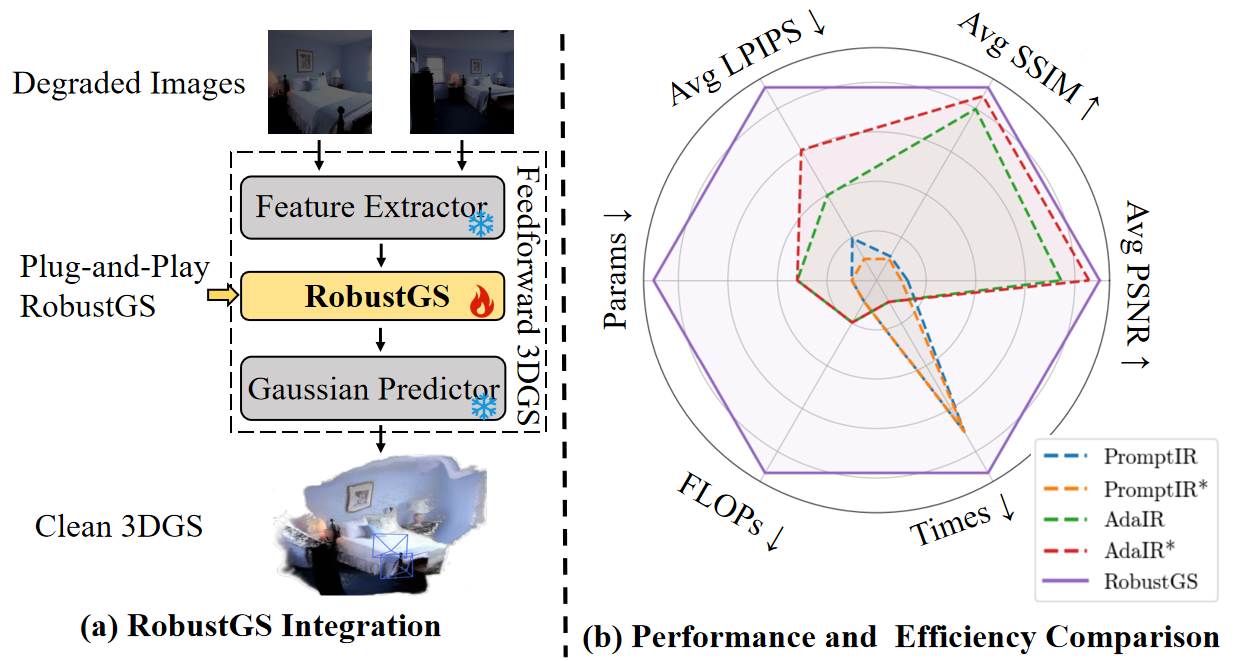
\includegraphics[width=1\columnwidth]{fig1.png} 
\caption{(a) Illustration of the proposed plug-and-play RobustGS integrated into the existing feedforward 3DGS pipeline to enhance robustness. (b) Our proposed RobustGS significantly outperforms existing methods in both visual quality and efficiency evaluations.}
\label{fig:overall}
\end{figure}



Recent progress in 3D reconstruction has seen a shift from neural implicit methods like NeRF to explicit representations such as 3D Gaussian Splatting (3DGS)~\cite{kerbl20233d}. 3DGS significantly advances the field by offering higher reconstruction fidelity and more efficient rendering compared to NeRF~\cite{mildenhall2021nerf}, thanks to its explicit and compact modeling of scene geometry and appearance. To improve scalability and speed, recent feedforward variants~\cite{szymanowicz2024splatter,tang2024lgm,charatan23pixelsplat,chen2024mvsplat,smart2024splatt3r,ye2024no} leverage neural networks to generate 3D Gaussian representations from a set of input images in a single pass, bypassing the need for per-scene optimization. However, these methods are typically trained and evaluated on curated datasets with clean, well-lit, and artifact-free images. In practical scenarios, input images often exhibit various degradations, such as noise, adverse environments, or challenging lighting conditions. Such degradations severely impact feature extraction and matching, leading to incomplete geometry, loss of detail, or distorted reconstructions~\cite{riegler2020free,liu2023robust,catley2024roguenerf,wu2024rafe,kwon2025r3evision}. Addressing these challenges is crucial for robust 3D reconstruction in unconstrained environments.



A straightforward solution is to apply image restoration techniques~\cite{chee2018airnet,liang2021swinir,su2022survey} to pre-process degraded inputs or to enhance rendered novel views. However, most restoration networks are designed to optimize perceptual quality in the image space, rather than ensuring geometric consistency across multiple views. This mismatch in objectives often results in artifacts and inconsistencies in the reconstructed 3D structure, ultimately undermining the fidelity and integrity of the scene representation~\cite{philip2019multi,jain2021putting,zhou2023sparsefusion,chen2024pgsr}. Furthermore, several recent studies have explored adapting 3DGS to handle degraded input~\cite{li2024chaos,chen2024deblur,cui2025luminance}. For example, WeatherGS~\cite{qian2024weathergs} focuses on scenes affected by rain and snow, while DehazeGS~\cite{ma2025dehazegs} only addresses hazy environments. Although effective in certain cases, these methods rely on per-scene optimization and are tailored to limited degradation types, restricting their generalization and scalability in scenarios with diverse and unknown degradations.



To address these challenges, we propose to enhance feature representations to improve the robustness of feedforward 3DGS methods under diverse and unknown degradations. Specifically, we introduce a plug-and-play, general-purpose feature enhancement module that can be seamlessly integrated into existing methods, as illustrated in Figure~\ref{fig:overall}(a). The proposed approach comprises two key components: a \NAMEdeg and a \NAMEfem. In particular, the \NAMEdeg module is designed to extract generic representations and distributions of multiple degradations from multi-view inputs, thereby enhancing degradation-awareness and improving the overall quality of 3D reconstruction. The extracted degradation representations are then used to guide the \NAMEfem, which enhances feature-level interactions across views through a semantic-aware state-space mechanism. This design enables the model to selectively propagate and aggregate semantically relevant features between views, thus improving the consistency and granularity of 3D reconstructions. By preserving the original 3DGS pipeline and eliminating the need for retraining, our method provides a simple yet powerful solution for robust feedforward 3D reconstruction under challenging and adverse conditions, as illustrated in Figure~\ref{fig:overall}(b). Our main contributions are as follows:


\begin{itemize}
    \item We propose a novel \NAMEdeg module that generically extracts various degradation representations from input images, thereby enhancing the network's degradation-awareness and robustness.

    \item We introduce a novel degradation-guided feature enhancement mechanism by injecting the degradation representations extracted by \NAMEdeg into the existing state-space model, enabling efficient and targeted enhancement of low-quality regions in the feature space.
    
    \item We design a semantic-aware multi-view interaction module, \NAMEfem, which aggregates features across different views based on semantic consistency, enabling fine-grained alignment and cross-view interaction in semantically similar regions.
    
    \item We implement a plug-and-play modular design, \NAMEall, that can be directly integrated into existing feedforward 3DGS methods. Our approach consistently improves reconstruction quality under six typical degradation types without requiring retraining of the original reconstruction pipeline.
\end{itemize}



\section{Related Work}
\subsection{feedforward 3DGS}

The advent of 3D Gaussian Splatting (3DGS)~\cite{kerbl20233d} has marked a major step forward in efficient 3D reconstruction and real-time novel view synthesis~\cite{lyu20243dgsr,chen2024optimizing,yang2024deformable,lu20243d,chen2025trends}. Compared to NeRF-based approaches~\cite{barron2021mip,muller2022instant,gao2022nerf,chen2023bidirectional,huang2023refsr}, 3DGS offers significant advantages in rendering speed and memory efficiency, making it highly suitable for interactive applications~\cite{kim20243dgs,liu2025artgs,khalid2025gaussianvae,gao2025towards}. Nevertheless, the original 3DGS and many of its extensions~\cite{fei20243d, wu2024recent, dalal2024gaussian} still rely on a large number of high-quality input images and require time-consuming optimization to achieve accurate geometry and appearance. To overcome these limitations, several feedforward pipelines have recently been proposed. For example,  PixelSplat~\cite{charatan23pixelsplat} leverages epipolar geometry to refine depth, enabling high-quality reconstruction from sparse views. NoPosSplat~\cite{ye2024no} further eliminates the need for camera poses and depth maps by exploiting cross-view feature correspondences, increasing flexibility in unconstrained scenarios. However, these methods typically assume clean, artifact-free multi-view inputs. In practice, images captured in the wild frequently suffer from degradations such as noise, blur, low light, or adverse weather, making the predicted Gaussian primitives unreliable and leading to degraded geometry, inconsistent colors, and visible artifacts in novel views. Despite these challenges, the robustness of feedforward 3DGS pipelines under degradations remains largely unexplored, significantly restricting their use in unconstrained environments.




\subsection{Image Restoration}

Low-level vision focuses on restoring degraded visual content and enhancing perceptual quality by removing noise, artifacts, or distortions~\cite{li2024efficient,li2025dual,peng2021ensemble,li2023cross,ren2024ultrapixel,yan2025textual,Li2023FCDFusion2}. It covers a wide range of tasks such as denoising, deblurring, deraining, and super-resolution, typically operating on individual images~\cite{peng2020cumulative,wang2023decoupling,peng2024lightweight,peng2024towards,wang2023brightness,xiao2025incorporating,li2024efficient2,li2025fouriersr,Li_2025_CVPR,Li2023FCDFusion}. Over the years, methods have evolved from convolution-based networks to transformer-based models~\cite{yi2021structure,yi2021efficient,peng2024efficient,conde2024real,li2024object,he2024dual}, with increasing capacity to handle diverse and complex degradations~\cite{peng2025directing,yi2025fine,he2024latent,he2024diffusion,he2025segment,he2025unfoldir}. As the field progresses~\cite{peng2025pixel,peng2025boosting,xiao2025event,li2025ustc,he2024multi,qi2025data,feng2025pmq,ren2021deep,xia2024s3mamba,li2023ntire,ren2024ninth,wang2025ntire}, recent methods have begun to consider more realistic degradation scenarios and adaptive strategies~\cite{he2023hqg,ren2025turbo2k,li2025frequency,zhao2024boosting,peng2024unveiling,he2025run,he2025reti,zheng2024odtrack,jin2024mipi,sun2024beyond}, such as blind restoration and degradation-aware modeling~\cite{ren2025triplane,ren2023towards,xiao2024event,zheng2023toward,di2025qmambabsr,ren2022dlformer,du2024fc3dnet}. Despite these advances, most approaches remain centered on single-view inputs and aim to optimize visual fidelity through pixel-wise or perceptual losses~\cite{li2024uniformly,zhao2023spike,zheng2022leveraging,gong2024beyond,zeng2024cross}. These pixel-level objectives, while effective for image enhancement~\cite{li2024loop,zheng2025decoupled,zheng2025towards,pan2025enhance,wu2025dropout,jiang2024dalpsr,ignatov2025rgb,gong2022person,lin2025phys4dgen}, may overlook deeper structural or semantic consistency crucial for downstream tasks like 3D reconstruction.


\subsection{3DGS in Degraded Scenes}

Most 3DGS methods are developed on clean images, while real-world scenes often suffer from degradations like rain, fog, or low light. Some recent approaches address these challenges through per-scene optimization~\cite{jin2024lighting,qiao2025restorgs,bui2025mobgs}, such as SRGS~\cite{feng2024srgs} for super-resolution, Deblurring 3DGS~\cite{lee2024deblurring} for deblurring, DehazeGS~\cite{ma2025dehazegs} for dehazing, and WeatherGS~\cite{qian2024weathergs} for adverse weather. However, these methods are limited to specific degradation types and require slow optimization for each scene. Although HQGS~\cite{linhqgs} extends to multiple degradations, it still relies on a sparse point cloud estimated by COLMAP. To our knowledge, no prior work has explored feature-level enhancement for robust, feedforward 3DGS under diverse and unknown degradations. Our work is the first to address this gap.


\begin{figure}[t]
\centering
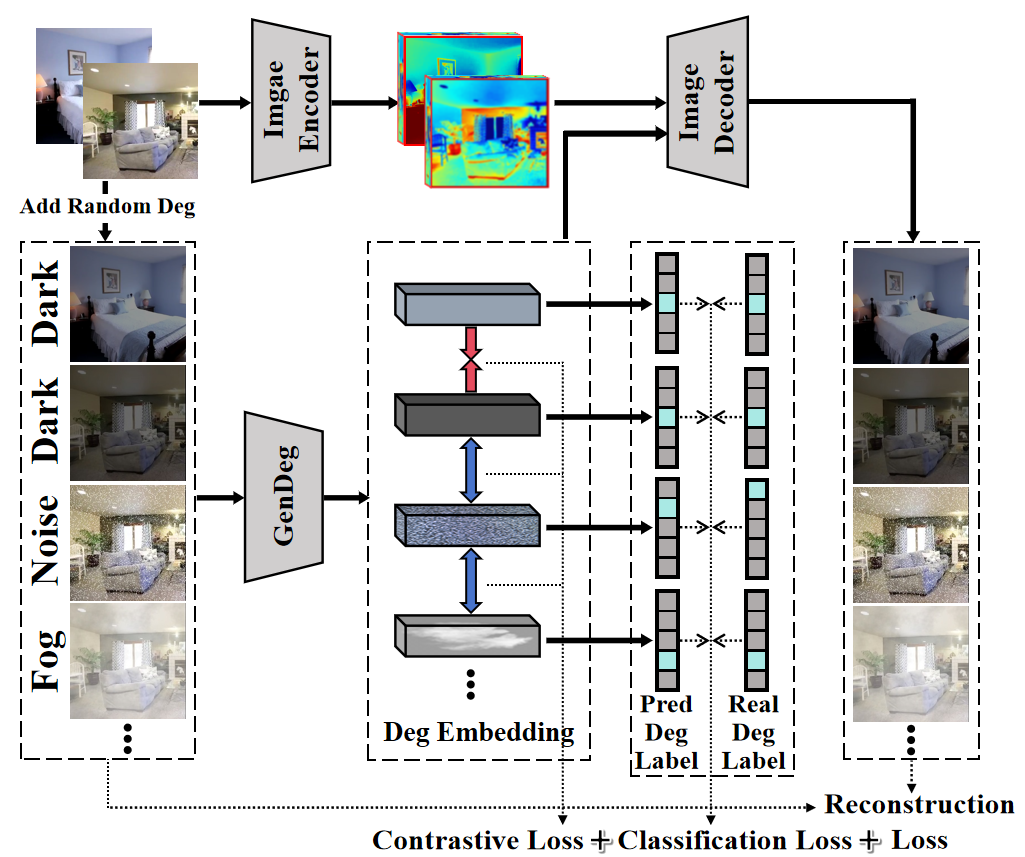
\includegraphics[width=1\columnwidth]{fig2.png} 
\caption{The carefully designed training pipeline for the Generalized Degradation Learner incorporates various supervision signals to fully extract the distribution and types of degradation signals, laying the foundation for our RobustGS.}


\label{fig:deg}
\end{figure}

\section{Proposed Method}
To enhance the robustness of feedforward 3DGS under degraded scenes, we propose a plug-and-play, unified feature enhancement framework, \NAMEall, that can be seamlessly integrated into existing reconstruction and rendering pipelines. Unlike methods tailored to specific degradation types, our approach offers a unified solution capable of simultaneously handles diverse degradations such as rain, snow, noise and low-light. Our method consists of two main stages. Firstly, we propose a \NAMEdeg that extracts compact and generalizable degradation representations from input images. Secondly, we design a \NAMEfem to leverage degradation representations for suppressing input artifacts while modeling semantic consistency and structural correspondence across views for feature enhancement. This design significantly enhances the recovery of degraded regions by leveraging both degradation cues and cross-view dependencies. As shown in Figure~\ref{fig:detail}(Left), the overall framework is efficient and broadly applicable to feedforward 3D reconstruction methods, leading to improved performance under a wide range of degradation conditions.




\subsection{Unified Degradation Representation Learning}

\begin{figure*}[t]
\centering

\includegraphics[width=1.0\textwidth]{fig3.png} % Reduce the figure size so that it is slightly narrower than the column. Don't use precise values for figure width.This setup will avoid overfull boxes.
\caption{Pipeline and key components of the proposed RobustGS framework. Left: The overall pipeline, in which RobustGS is integrated into the standard feedforward 3DGS architecture. (a) The architecture of \NAMEfem (MV-SSEM), consisting of multiple Feature Enhancement Blocks (FEBs). (b) Multi-view semantic guidance module, where semantic prompts are extracted across views and spatial tokens are reordered accordingly. (c) Feature enhancement via the  State-Space Module (SSM), jointly guided by degradation embeddings and semantic prompts.}
\label{fig:detail}
\end{figure*}

To enable robust all-in-one enhancement across diverse degradation types in the feature space, it is essential for the model to perceive the degradation characteristics present in the input. Therefore, we propose a \textit{\NAMEdeg} (GenDeg) that distills high-level degradation information into a compact latent, as shown in Figure~\ref{fig:deg}. This implicit representation provides a global degradation context to guide subsequent feature enhancement.

GenDeg is implemented as a neural degradation-aware encoder, which processes the degraded image $I_{\mathrm{deg}}$ to generate a degradation embedding $z_{\mathrm{deg}} \in \mathbb{R}^{C \times 1}$. $z_{\mathrm{deg}}$ captures degradation-specific cues to enable condition-aware enhancement in downstream stages. To train GenDeg effectively, we design an auxiliary reconstruction pipeline. Specifically, a \textbf{Content Encoder} processes the clean counterpart $I_{\mathrm{clean}}$ to produce content features, which are then fused with $z_{\mathrm{deg}}$ via a \textbf{Content Decoder} to reconstruct the original degraded image $\hat{I}_{\mathrm{deg}}$. This training mechanism enables $z_{\mathrm{deg}}$ to be learned in a self-supervised pattern, such that it carries sufficient degradation cues to reconstruct the observed corrupted input when combined with clean content.

Instead of relying on explicit degradation labels, the degradation embedding $z_{\mathrm{deg}}$ is learned as an \textit{implicit representation}, capturing underlying degradation characteristics directly from the pixel distribution. This latent representation encapsulates high-level degradation semantics (\textit{e.g.}, rain, noise, fog) in a latent space, which enables generalization across degradation types. To encourage the embedding to capture degradation-relevant features, we optimize the module with two complementary objectives:


\paragraph{Reconstruction Loss.} 
To ensure that the degradation embedding $z_{\mathrm{deg}}$ effectively captures the intrinsic degradation characteristics, we train the decoder to reconstruct the original degraded image. The supervision combines both pixel-wise and perceptual losses:

\begin{equation}
    \mathcal{L}_{\mathrm{rec}} =  \lambda\| \hat{I}_{\mathrm{deg}} - I_{\mathrm{deg}} \|_1 +  \mathcal{L}_{\mathrm{perc}}(\hat{I}_{\mathrm{deg}}, I_{\mathrm{deg}}).
\end{equation}
where $\mathcal{L}_{\mathrm{perc}}$ is a perceptual loss computed from a pre-trained VGG network and \(\lambda\) is empirically set to 0.1. The $\ell_1$ term enforces pixel-level fidelity, while the perceptual term emphasizes high-level semantic and structural similarity. By minimizing this reconstruction loss, we indirectly encourage GenDeg to extract embeddings that faithfully encapsulate degradation-specific cues, since only an informative $z_{\mathrm{deg}}$ can guide the decoder to synthesize a visually and semantically consistent degraded image.


\paragraph{Contrastive Loss.} To enhance the discriminability of the embedding space, we adopt a contrastive objective:
\begin{equation}
    \mathcal{L}_{\mathrm{con}} = -\log \frac{\exp(\mathrm{sim}(z_i, z_j)/\tau)}{\sum_{k \ne i} \exp(\mathrm{sim}(z_i, z_k)/\tau)}.
\end{equation}
where $\mathrm{sim}(\cdot,\cdot)$ denotes cosine similarity, and $(z_i, z_j)$ is a positive pair with the same degradation type. This encourages embeddings of similar degradations to be closer while pushing dissimilar types apart.

\paragraph{Classification Loss.} To further regularize the learning of $z_{\mathrm{deg}}$, we attach a lightweight classifier after the embedding to predict the degradation type. Although not used during inference, this auxiliary operation encourages the embedding to capture more explicit degradation cues. The supervision is provided by a cross-entropy loss:
\begin{equation}
\mathcal{L}_{\mathrm{cls}} = \mathrm{CrossEntropy}(f_{\mathrm{cls}}(z_{\mathrm{deg}}), y_{\mathrm{deg}}).
\end{equation}
The overall training objective is defined as $\mathcal{L} = \lambda_1 \mathcal{L}_{\mathrm{rec}} + \lambda_2 \mathcal{L}_{\mathrm{con}} + \lambda_3 \mathcal{L}_{\mathrm{cls}}$, with the weights are empirically set to $\lambda_1 = 1.0$, $\lambda_2 = 0.5$, and $\lambda_3 = 0.3$.



Through the joint optimization of $\mathcal{L}_{\mathrm{rec}}$, $\mathcal{L}_{\mathrm{con}}$, and $\mathcal{L}_{\mathrm{cls}}$, the embedding module learns to represent degradation in a way that is reconstructive, discriminative, and semantically aligned with degradation categories. This degradation-aware signal serves as a high-level conditioning cue for feature-level enhancement in downstream modules.

\subsection{Multi-view Feature Enhancement}




\begin{table*}[ht]
% \begin{center}
\centering
\setlength{\tabcolsep}{1.1mm}
\begin{tabular}{l|lll|lll|lll|lll}
\toprule
& \multicolumn{3}{c|}{Brightness}                     & \multicolumn{3}{c|}{Fog}                            & \multicolumn{3}{c|}{Contrast}                       & \multicolumn{3}{c}{Snow}                                                                                           \\ \cmidrule(lr){2-13}
           & PSNR           & SSIM            & LPIPS           & PSNR           & SSIM            & LPIPS           & PSNR           & SSIM            & LPIPS           & PSNR                                 & SSIM                                 & LPIPS                                \\ \midrule
Pixelsplat & 15.03          & 0.7919          & 0.1753          & 14.88          & 0.7321          & 0.2044          & 18.40          & 0.7195          & 0.2453          & 19.15                                & 0.5809                               & 0.4297                               \\
PromptIR   & 14.31          & 0.7664          & 0.1797          & \underline{21.50}          & \underline{0.8160}          & 0.2043          & 18.30          & 0.7161          & 0.2440          & 19.87                                & 0.6151                               & 0.4089                               \\
PromptIR\ding{72}   & 16.99          & 0.7811          & 0.1897          & 21.33          & 0.8100          & 0.2031          & \underline{21.80}          & \underline{0.8047}          & \underline{0.2197}         & \textbf{21.46}                       & \textbf{0.6794}                      & \textbf{0.3844}                      \\
PromptIR\ding{73}   & \underline{23.91}          & 0.8431          & 0.1645        & 20.35          & 0.8034          & 0.2145          & 16.29          & 0.6770          & 0.2557          & 17.13                                & 0.6085                               & 0.4404                               \\
AdaIR      & 14.78          & 0.7817          & 0.1775          & 20.91          & 0.8146          & \underline{0.1994}          & 18.37          & 0.7197          & 0.2457          & 19.72                                & 0.6151                               & 0.4049                              \\
AdaIR\ding{72}      & 23.59          & \underline{0.8501}          & \textbf{0.1527} & 15.40          & 0.7115          & 0.2709          & 16.88          & 0.7064          & 0.2315          & 16.29                                & 0.5908                               & 0.4458                               \\
AdaIR\ding{73}      & 23.45          & 0.8493          & 0.1631          & 15.54          & 0.6018          & 0.4518          & 15.37          & 0.6750          & 0.2560          & 15.54                                & 0.6018                               & 0.4518                               \\
RobustGS   & \textbf{24.87} & \textbf{0.8512} & \underline{0.1617}          & \textbf{21.52} & \textbf{0.8209} & \textbf{0.1974} & \textbf{22.05} & \textbf{0.8062} & \textbf{0.2147} & \underline{20.78}                                & \underline{0.6495}                               & \underline{0.4003} \\ \midrule \midrule

& \multicolumn{3}{c|}{Rain}                           & \multicolumn{3}{c|}{Impulse noise}                 & \multicolumn{3}{c|}{\textbf{Average performance}}            & \multicolumn{3}{c}{Complexity}                                                                                     \\  \cmidrule(lr){2-13}
           & PSNR           & SSIM            & LPIPS           & PSNR           & SSIM            & LPIPS           & PSNR           & SSIM            & LPIPS           & FLOPs                                & Params                               & time(ms)                             \\ \midrule
Pixelsplat & 19.62          & 0.7325          & 0.3036          & 14.08          & 0.7578          & 0.2626          & 16.86          & 0.7191          & 0.2701          & \multicolumn{1}{c}{\textbackslash{}} & \multicolumn{1}{c}{\textbackslash{}} & \multicolumn{1}{c}{\textbackslash{}} \\
PromptIR   & 21.65          & 0.7473          & 0.2921          & 14.33          & 0.7633          & 0.2610          & 18.33          & 0.7374          & 0.2650         & \multicolumn{1}{c}{43.28 G} & \multicolumn{1}{c}{35.59 M} & \multicolumn{1}{c}{\underline{91.68 ms}}
                               \\
PromptIR\ding{72}   & 21.88          & \underline{0.7826}          & 0.2662        & 20.71          & 0.8054       & 0.2424          & \underline{20.69}          & \underline{0.7772}          & \underline{0.2509}          & \multicolumn{1}{c}{43.28 G} & \multicolumn{1}{c}{35.59 M} & \multicolumn{1}{c}{91.68 ms}                                \\
PromptIR\ding{73}   & 21.30          & 0.7779          & 0.2687          & \underline{21.67}          & \underline{0.8109}          & 0.2529          & 20.11          & 0.7535          & 0.2661          & \multicolumn{1}{c}{43.28 G} & \multicolumn{1}{c}{35.59 M} & \multicolumn{1}{c}{91.68 ms} \\
AdaIR      & 21.02          & 0.7383          & 0.3020          & 14.37          & 0.7604          & 0.2618          & 18.20          & 0.7383          & 0.2652          & \multicolumn{1}{c}{\underline{40.54 G}} & \multicolumn{1}{c}{\underline{28.78 M}} & \multicolumn{1}{c}{226.01 ms}
                            \\
AdaIR\ding{72}      & \textbf{23.06} & \textbf{0.8150} & \textbf{0.2111} & 20.37          & 0.8045          & \underline{0.2297}          & 19.26          & 0.7464          & 0.2570         & \multicolumn{1}{c}{40.54 G} & \multicolumn{1}{c}{28.78 M} & \multicolumn{1}{c}{226.01 ms}                              \\
AdaIR\ding{73}      & 19.30          & 0.7576          & 0.2962          & 20.66          & 0.8013          & 0.2570          & 18.31          & 0.7145          & 0.3127          & \multicolumn{1}{c}{40.54 G} & \multicolumn{1}{c}{28.78 M} & \multicolumn{1}{c}{226.01 ms} \\

RobustGS   & \underline{22.65}          & 0.7809          & \underline{0.2652}          & \textbf{22.03} & \textbf{0.8129} & \textbf{0.2267} & \textbf{22.32} & \textbf{0.7869} & \textbf{0.2443} & \multicolumn{1}{c}{\textbf{20.51 G}}                              & \multicolumn{1}{c}{\textbf{10.83 M}}                              & \multicolumn{1}{c}{\textbf{49.10ms}}
\\ \bottomrule
\end{tabular}

\caption{Comparison of performance and computational complexity with existing methods across various degradation scenarios. Bold indicates the best performance, while underline denotes the second-best.}
\label{table1}
% \end{center}
\end{table*}


To address feature degradation in the feedforward 3DGS pipeline, we introduce \NAMEfem. Instead of modifying the 3DGS backbone, we design a standalone, plug-and-play enhancement block, as shown in Figure~\ref{fig:detail}(a). Our method aims to enhance the quality of intermediate features extracted from degraded multi-view images, thereby providing cleaner and more reliable features for downstream 3D reconstruction. Specifically, degradation embeddings extracted from GenDeg are used to explicitly guide the feature enhancement process. By integrating these degradation priors into a carefully designed multi-scale framework, the network becomes aware of the type and severity of degradation at different spatial resolutions, enabling more effective feature enhancement.

Degradation in images is typically distributed across the entire image. Therefore, effective removal of degradation and feature fusion requires network capable of capturing global context while maintaining computational efficiency. To address this, we adopt a set of State Space Model (SSM) based blocks, which enable more effective representation and enhancement of degraded features through global context modeling. The general form of a continuous-time Linear State Space Model is defined as:
\begin{equation}
    \dot{h}(t) = A h(t) + B x(t), \
    y(t) = C h(t) + D x(t),
\end{equation}
where $x(t)$ is the input signal, $h(t)$ is the hidden state, and $y(t)$ is the output at time $t$. The matrices $A$, $B$, $C$, and $D$ parameterize the system dynamics and output mapping. This formulation captures the influence of both the internal system state and external input on the output in a continuous, recursive manner. To adapt the continuous model to discrete image representations, we discretize the system using matrix exponentials:
\begin{equation}
    \overline{A} = \exp(\Delta A), \
    \overline{B} = (\Delta A)^{-1} (\exp(\Delta A) - I) \Delta B,
\end{equation}
where $\Delta$ is a learnable step size and $I$ is the identity matrix.The resulting discrete-time SSM is updated as:
\begin{equation}
    h_k = \overline{A} h_{k-1} + \overline{B} x_k, \
    y_k = C h_k + D x_k.
\end{equation}
This formulation allows directional and position-aware feature modeling by integrating the current input $x_k$ with the memory state $h_{k-1}$ ~\cite{guo2024mambair}. 


To achieve robust all-in-one feature enhancement under unknown degradations, we introduce a degradation-aware modulation mechanism that dynamically adjusts the selective scan process based on degradation characteristics. Since the degradation type and severity are typically unknown during inference, a unified and learnable guidance signal is required to modulate the enhancement process accordingly. Based on this, we utilize the degradation embedding \( z_{\text{deg}} \), a compact vector extracted from GenDeg, which encodes high-level semantics of the degradation. As shown in Figure~\ref{fig:detail}(c), the degradation embedding primarily modulates the input projection matrix \( B \), which governs how degraded input tokens are integrated into the hidden state. The embedding \( z_{\text{deg}} \) also modulates the output projection \( C \) and the update step size \( \Delta \), enabling global degradation-aware adaptation in the selective scan process. Specifically, the degradation embedding is fed into three separate lightweight MLPs (\(\phi\)) to generate modulation coefficients, which are then applied via element-wise multiplication:
\begin{equation}
    W_{\text{mod}} = W \odot \phi_W(z_{\text{deg}}), \quad W \in \{B, C, \Delta\}.
\end{equation}
This degradation-guided modulation enables the selective scan to adapt its dynamic behavior to the degradation characteristics of the input. By conditioning the enhancement parameters on \( z_{\text{deg}} \), the model can restore degraded regions and preserve semantic structures better across diverse scenarios. This design enables unified feature enhancement without requiring degradation-specific tuning, making the module generalizable for different degradation scenes.



\begin{figure*}[t]
\centering
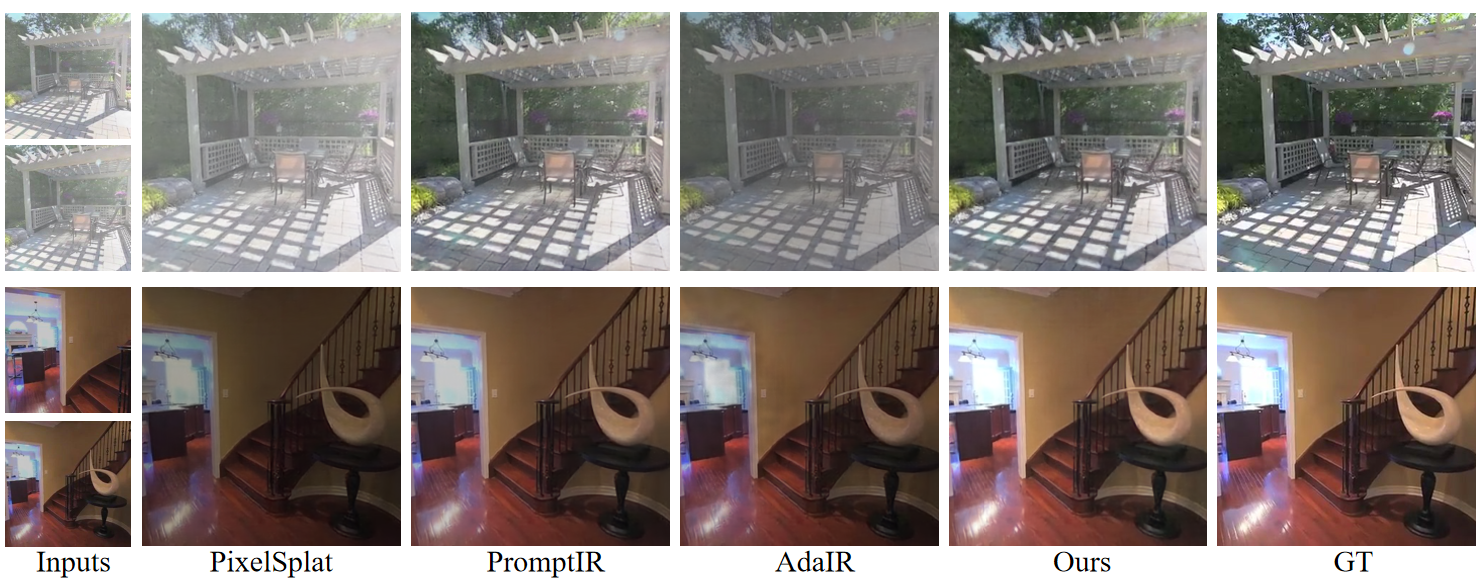
\includegraphics[width=1.0\textwidth]{fig4.png} 
\caption{Qualitative comparison. The visual quality of our method outperforms restore before reconstruct methods. Visual examples in the first and second rows correspond to foggy and dark degradation scenes, respectively.}
\label{fig:vis_rgb_1}
\end{figure*}

\begin{table*}[ht!]
\centering

\begin{tabular}{l|cccccccc}
\toprule
     & mvsplat & PromptIR & PromptIR\ding{72} & PromptIR\ding{73} & AdaIR  & AdaIR\ding{72}  & AdaIR\ding{73}  & RobustGS \\ \midrule
Avg PSNR & 17.20    & 18.57    & 20.04    & 19.31    & 18.43  & 19.58  & 18.14  & \textbf{21.48}    \\
Avg SSIM & 0.7307  & 0.7512   & 0.7726   & 0.7476   & 0.7499 & 0.7601 & 0.7425 & \textbf{0.7851}  
\\ \bottomrule
\end{tabular}
\caption{Average Performance Comparison on the MVSplat backbone. More details are presented in Appendix.}

\label{table2}
\end{table*}


To mitigate feature loss caused by degradation, we leverage the complementary information across multi-view images and propose a semantic-aware consistency enhancement mechanism, inspired by the semantic-aware design in MambaIRv2~\cite{guo2025mambairv2}. The key motivation is to encourage feature interactions across views by reorganizing tokens based on their latent semantics, as shown in Figure~\ref{fig:detail}(b). Concretely, we first extract the semantic representations from the feature map using a learnable projection network. Given a feature map $F \in \mathbb{R}^{N \times d}$ containing $N$ tokens, we generate semantic embeddings $\mathbf{E} = \{\mathbf{e}_1, \mathbf{e}_2, \dots, \mathbf{e}_N\}$, where $\mathbf{E} = f_{\text{sem}}(F)$, $\mathbf{e}_i$ represents the semantic feature of token $i$ and $f_{\text{sem}}(\cdot)$ denotes the global semantic encoder. We then introduce a learnable semantic pool $\mathcal{P} = \{\mathbf{p}_1, \mathbf{p}_2, \dots, \mathbf{p}_K\}$ composed of $K$ semantic prototypes. The similarity between each token’s semantic embedding and the prototypes is computed, followed by a Gumbel-Softmax to obtain a discrete semantic assignment:
\begin{equation}
    \mathbf{w}_i = \mathrm{GumbelSoftmax}(\mathrm{sim}(\mathbf{e}_i, \mathcal{P})).
\end{equation}
where $\mathbf{w}_i \in \mathbb{R}^K$ denotes the categorical distribution over semantic classes, and $\mathrm{sim}(\cdot)$ is a similarity function. Based on this semantic distribution, we reorder all tokens so that those with similar semantics are spatially grouped. This reorganization promotes inter-view interaction by aligning semantically related content, and further alleviates long-range forgetting problems in SSM model.


Moreover, we modulate the scan parameters using semantic-aware signals, as shown in Figure~\ref{fig:detail}(c). Each token’s semantic distribution $\mathbf{w}_i$ is used to adaptively adjust the scanning matrix $C$ as follows:
\begin{equation}
    C_i^{\text{mod}} = C + \sum_{k=1}^K w_{ik} \cdot \mathbf{p}_k.
\end{equation}
where $C_i^{\text{mod}}$ is the modulated scanning weight for token $i$. This modulation allows the scan operation to become more sensitive to semantic context, enabling a more effective feature enhancement pipeline. To further facilitate consistent information propagation, we introduce a cross-stage feedback mechanism in the decoder: the modulation matrix generated at a lower-resolution stage is passed to the next stage as state information to guide the selective scan. This design helps retain global structural cues from earlier stages and improves the quality of feature reconstruction at higher resolutions.





\section{Experiment and Analysis}
\subsection{Experiment Setting}
\subsubsection{Datasets and implementation details.}

We first train \NAMEdeg on the DIV2K dataset~\cite{wang2021real}, a high-quality image dataset that is widely used for degradation simulation. Following the degradation protocol of RobustSAM ~\cite{chen2024robustsam}, we synthesize diverse low-quality variants to enable the learning of robust and generalizable degradation priors. Subsequently, we train \NAMEfem on the RealEstate10K (RE10K) dataset~\cite{zhou2018stereo}, using the same degradation synthesis protocol in GenDeg stage. RE10K provides multi-view video sequences along with camera poses estimated via structure-from-motion (SfM) using COLMAP~\cite{7780814}. For consistency with existing feedforward 3DGS pipelines and to ensure fair comparisons, we adopt the official training and testing splits used in prior work and train our model at a resolution of 256×256. Notably, we observe that using only approximately 10\% of the RE10K training data is sufficient to achieve competitive results, highlighting the efficiency and generalization capability of our network. Further implementation details are provided in the appendix.



\subsubsection{Evaluation metrics and compared methods.}
We evaluate the quality of novel view synthesis using PSNR, SSIM~\cite{wang2004image}, and LPIPS~\cite{zhang2018unreasonable}. To assess the effectiveness of our method, we compare it against two state-of-the-art image restoration baselines, PromptIR~\cite{potlapalli2023promptir} and AdaIR~\cite{cui2024adair}, under three settings: (1) using official pretrained weights where restoration precedes 3D reconstruction; (2) retraining the restoration models under our degradation settings followed by reconstruction (\ding{72}); and (3) reversing the pipeline order such that reconstruction precedes restoration on rendered images (\ding{73}). Additionally, we compare the parameters, FLOPs, and runtime to evaluate their efficiency and deployment feasibility. 





\subsection{Quantitative Results}



\subsubsection{Quantitative comparisons.}

As presented in Table~\ref{table1}, the integration of the RobustGS module into the feedforward 3DGS framework Pixelsplat brings consistent and significant performance enhancements across diverse degradation scenarios and evaluation metrics. In comparison to state-of-the-art general-purpose image restoration methods, whether applied prior to reconstruction or post-rendering, our approach demonstrates clear superiority in terms of average PSNR, SSIM, and LPIPS. To further showcase the versatility of RobustGS, we integrate it into another prominent feedforward 3DGS backbone, MVSplat. As illustrated in Table~\ref{table2}, RobustGS consistently achieves competitive performance across all metrics, reaffirming its robustness and adaptability to varying architectures and conditions.

\begin{figure}[t]
\centering
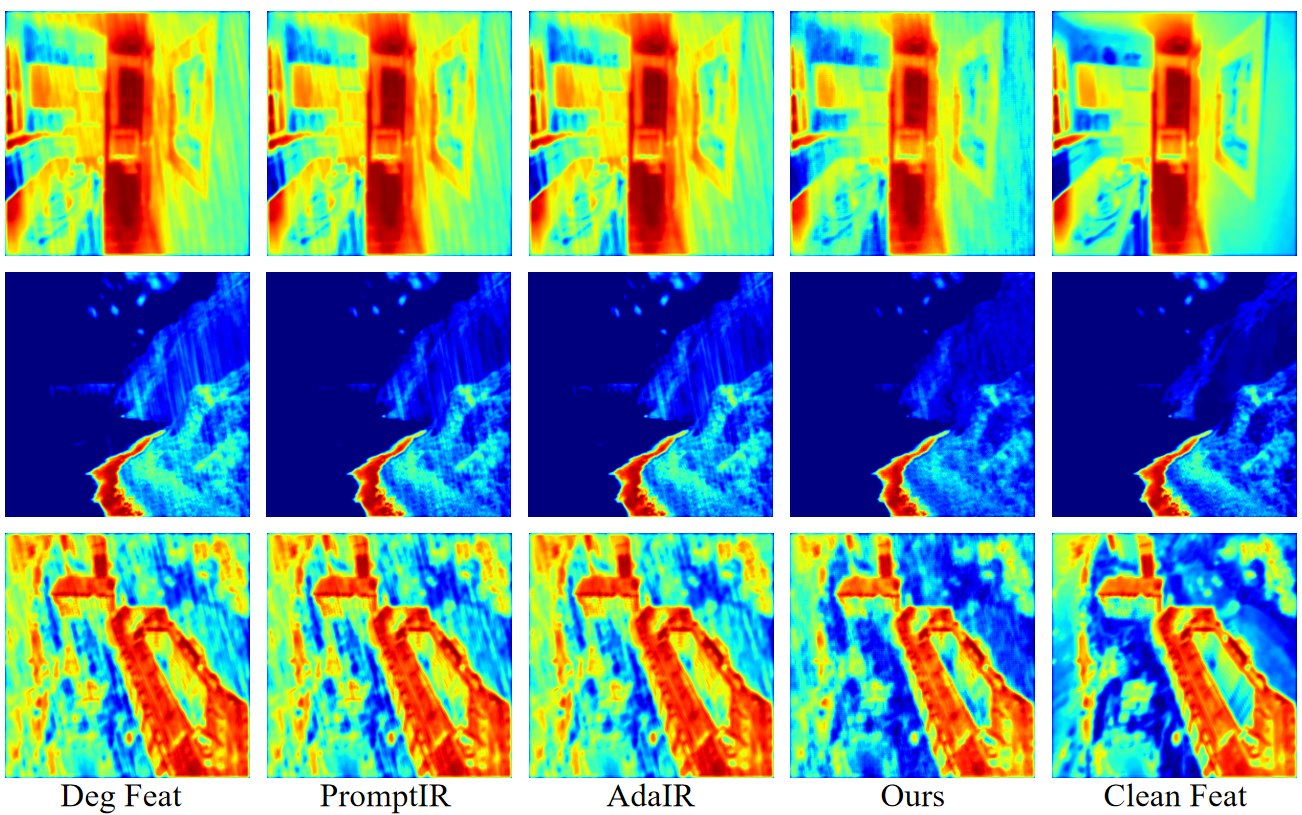
\includegraphics[width=1\columnwidth]{fig5.png} % Reduce the figure size so that it is slightly narrower than the column. Don't use precise values for figure width.This setup will avoid overfull boxes.
\caption{Feature map visualization under rain scenes.}
\label{fig:vis_feat}
\end{figure}


\begin{table}[ht]
\centering
% \setlength{\tabcolsep}{0.9mm}
\begin{tabular}{cccc|ll}
\toprule

Deg emb & Deg→SSM & SR & MV & PSNR & SSIM \\ \midrule
                &         & \checkmark                & \checkmark         & 21.52 & 0.7803 \\
\checkmark              &         & \checkmark                &\checkmark          & 21.71 & 0.7846 \\
\checkmark               & \checkmark       &                  & \checkmark          & 22.05 & 0.7850  \\
\checkmark               & \checkmark       & \checkmark                &            & 21.96 & 0.7794 \\
\checkmark               & \checkmark       & \checkmark                & \checkmark          & \textbf{22.32} & \textbf{0.7869}
\\ \bottomrule
\end{tabular}
\caption{Ablation study.}

\label{table3}
\end{table}

\subsubsection{Complexity comparisons.}  

In addition to evaluating performance metrics, we compare the computational complexity of different methods, including the number of parameters, FLOPs, and runtime, with FLOPs and runtime measured using two input images of size $64 \times 64$. As shown in Table~\ref{table1}, the RobustGS module not only delivers substantial performance gains but also achieves a lower computational cost compared to existing image restoration approaches. Furthermore, as a plug-and-play solution that requires no retraining of the original 3DGS model, RobustGS offers an efficient and practical approach to enhancing 3D reconstruction across diverse degradation scenarios.

\subsection{Qualitative Results}



Figure~\ref{fig:vis_rgb_1} presents qualitative comparisons under two representative degradation scenarios, dark and fog, between our RobustGS and a pipeline combining representative IR methods with PixelSplat reconstruction. In these pipelines, IR methods are applied to enhance input images before 3D reconstruction. While effective for single-view enhancement, these methods fail to ensure geometric consistency across multiple views, often leading to rendering artifacts in reconstructed images. For instance, in the dark scenario (second column), AdaIR introduces noticeable black blob artifacts on the wall due to inconsistent restoration across views, resulting in erroneous geometry. In contrast, RobustGS explicitly models cross-view consistency at the feature level, effectively mitigating such artifacts and producing stable, visually reliable reconstructions. To further validate its effectiveness, we visualize intermediate feature maps in Figure~\ref{fig:vis_feat}. The enhanced features generated by RobustGS successfully remove most degradation artifacts from the original features, yielding clearer structures and more complete semantic representations.


\subsection{Ablation Study}
In this section, we conduct ablation studies to evaluate the contributions of each key component in RobustGS. We first analyze the impact of the \NAMEdeg and compare two integration strategies: direct concatenation of the degradation embedding versus injection into the SSM. Additionally, we examine the effects of semantic-guided token reordering in \NAMEfem and the role of multi-view interaction versus single-view processing. As summarized in Table~\ref{table3}, the full design consistently achieves the best performance, where SR represents semantic reorder and MV denotes multi-view. To validate GenDeg, we visualize its degradation embeddings using t-SNE, where embeddings for different degradation types form distinct clusters, separated from clean images, demonstrating their discriminative power and generalizability. Further ablation results are included in the Appendix.


\begin{figure}[t]
\centering
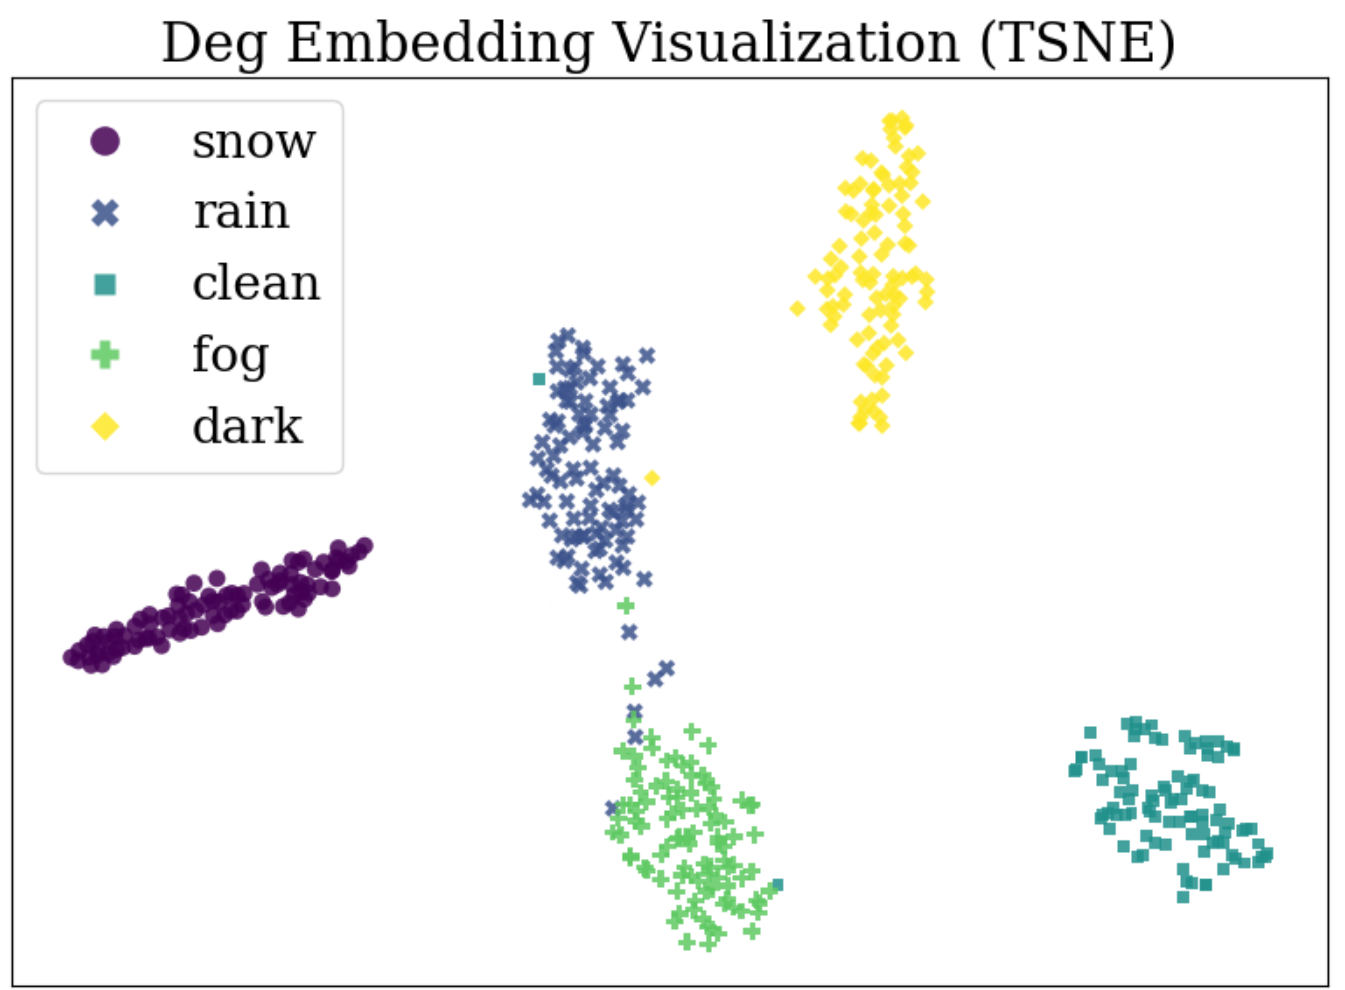
\includegraphics[width=0.8\columnwidth]{fig6.png}
\caption{t-SNE visualization.}

\label{fig:vis_tsne}
\end{figure}

\section{Conclusion}

This paper presents RobustGS, a general and efficient feature enhancement module designed to improve the robustness of feedforward 3D Gaussian Splatting (3DGS) methods under challenging degraded conditions. By introducing the Generalized Degradation Learner to extract compact and generalizable degradation representations and the Multi-View State-Space Enhancement Module to leverage degradation-aware cues and semantic consistency for feature enhancement, RobustGS addresses the limitations of existing 3DGS approaches in handling degraded multi-view inputs. Extensive experiments demonstrate that RobustGS, integrated seamlessly into existing pipelines without requiring retraining, consistently achieves state-of-the-art performance across multiple degradation scenarios, significantly improving reconstruction quality in terms of PSNR, SSIM, and LPIPS metrics while maintaining lower computational complexity.


\clearpage

\bibliography{aaai2026}

\clearpage
%File: anonymous-submission-latex-2026.tex
% \documentclass[letterpaper]{article} % DO NOT CHANGE THIS
% \usepackage[submission]{aaai2026}  % DO NOT CHANGE THIS
% \usepackage{times}  % DO NOT CHANGE THIS
% \usepackage{helvet}  % DO NOT CHANGE THIS
% \usepackage{courier}  % DO NOT CHANGE THIS
% \usepackage[hyphens]{url}  % DO NOT CHANGE THIS
% \usepackage{graphicx} % DO NOT CHANGE THIS
% \urlstyle{rm} % DO NOT CHANGE THIS
% \def\UrlFont{\rm}  % DO NOT CHANGE THIS
% \usepackage{natbib}  % DO NOT CHANGE THIS AND DO NOT ADD ANY OPTIONS TO IT
% \usepackage{caption} % DO NOT CHANGE THIS AND DO NOT ADD ANY OPTIONS TO IT
\frenchspacing  % DO NOT CHANGE THIS
\setlength{\pdfpagewidth}{8.5in} % DO NOT CHANGE THIS
\setlength{\pdfpageheight}{11in} % DO NOT CHANGE THIS
%
% These are recommended to typeset algorithms but not required. See the subsubsection on algorithms. Remove them if you don't have algorithms in your paper.
% \usepackage{algorithm}
% \usepackage{algorithmic}
% \usepackage{amssymb}
% \usepackage{amsmath}
% \usepackage{xcolor}
% \newcommand{\pl}[1]{\textcolor{blue}{#1}}

% \usepackage{multirow} 
% \usepackage{booktabs}
% \usepackage{xspace}
% \usepackage{pifont}
% \newcommand{\NAMEfem}{Multi-View State-Space Enhancement Module\xspace}
% \newcommand{\NAMEdeg}{Generalized Degradation Learner\xspace}
% \newcommand{\NAMEall}{RobustGS\xspace}

% %
% % These are are recommended to typeset listings but not required. See the subsubsection on listing. Remove this block if you don't have listings in your paper.
% \usepackage{newfloat}
% \usepackage{listings}
% \DeclareCaptionStyle{ruled}{labelfont=normalfont,labelsep=colon,strut=off} % DO NOT CHANGE THIS
% \lstset{%
% 	basicstyle={\footnotesize\ttfamily},% footnotesize acceptable for monospace
% 	numbers=left,numberstyle=\footnotesize,xleftmargin=2em,% show line numbers, remove this entire line if you don't want the numbers.
% 	aboveskip=0pt,belowskip=0pt,%
% 	showstringspaces=false,tabsize=2,breaklines=true}
% \floatstyle{ruled}
% \newfloat{listing}{tb}{lst}{}
% \floatname{listing}{Listing}
% %
% % Keep the \pdfinfo as shown here. There's no need
% % for you to add the /Title and /Author tags.
% \pdfinfo{
% /TemplateVersion (2026.1)
% }


% DISALLOWED PACKAGES
% \usepackage{authblk} -- This package is specifically forbidden
% \usepackage{balance} -- This package is specifically forbidden
% \usepackage{color (if used in text)
% \usepackage{CJK} -- This package is specifically forbidden
% \usepackage{float} -- This package is specifically forbidden
% \usepackage{flushend} -- This package is specifically forbidden
% \usepackage{fontenc} -- This package is specifically forbidden
% \usepackage{fullpage} -- This package is specifically forbidden
% \usepackage{geometry} -- This package is specifically forbidden
% \usepackage{grffile} -- This package is specifically forbidden
% \usepackage{hyperref} -- This package is specifically forbidden
% \usepackage{navigator} -- This package is specifically forbidden
% (or any other package that embeds links such as navigator or hyperref)
% \indentfirst} -- This package is specifically forbidden
% \layout} -- This package is specifically forbidden
% \multicol} -- This package is specifically forbidden
% \nameref} -- This package is specifically forbidden
% \usepackage{savetrees} -- This package is specifically forbidden
% \usepackage{setspace} -- This package is specifically forbidden
% \usepackage{stfloats} -- This package is specifically forbidden
% \usepackage{tabu} -- This package is specifically forbidden
% \usepackage{titlesec} -- This package is specifically forbidden
% \usepackage{tocbibind} -- This package is specifically forbidden
% \usepackage{ulem} -- This package is specifically forbidden
% \usepackage{wrapfig} -- This package is specifically forbidden
% DISALLOWED COMMANDS
% \nocopyright -- Your paper will not be published if you use this command
% \addtolength -- This command may not be used
% \balance -- This command may not be used
% \baselinestretch -- Your paper will not be published if you use this command
% \clearpage -- No page breaks of any kind may be used for the final version of your paper
% \columnsep -- This command may not be used
% \newpage -- No page breaks of any kind may be used for the final version of your paper
% \pagebreak -- No page breaks of any kind may be used for the final version of your paperr
% \pagestyle -- This command may not be used
% \tiny -- This is not an acceptable font size.
% \vspace{- -- No negative value may be used in proximity of a caption, figure, table, section, subsection, subsubsection, or reference
% \vskip{- -- No negative value may be used to alter spacing above or below a caption, figure, table, section, subsection, subsubsection, or reference

\setcounter{secnumdepth}{0} %May be changed to 1 or 2 if section numbers are desired.

% The file aaai2026.sty is the style file for AAAI Press
% proceedings, working notes, and technical reports.
%

% Title

% Your title must be in mixed case, not sentence case.
% That means all verbs (including short verbs like be, is, using,and go),
% nouns, adverbs, adjectives should be capitalized, including both words in hyphenated terms, while
% articles, conjunctions, and prepositions are lower case unless they
% directly follow a colon or long dash
\title{RobustGS: Unified Boosting of Feedforward 3D Gaussian Splatting under Low-Quality Conditions}
\author{
    %Authors
    % All authors must be in the same font size and format.
    Written by AAAI Press Staff\textsuperscript{\rm 1}\thanks{With help from the AAAI Publications Committee.}\\
    AAAI Style Contributions by Pater Patel Schneider,
    Sunil Issar,\\
    J. Scott Penberthy,
    George Ferguson,
    Hans Guesgen,
    Francisco Cruz\equalcontrib,
    Marc Pujol-Gonzalez\equalcontrib
}
% \affiliations{
%     %Afiliations
%     \textsuperscript{\rm 1}Association for the Advancement of Artificial Intelligence\\
%     % If you have multiple authors and multiple affiliations
%     % use superscripts in text and roman font to identify them.
%     % For example,

%     % Sunil Issar\textsuperscript{\rm 2},
%     % J. Scott Penberthy\textsuperscript{\rm 3},
%     % George Ferguson\textsuperscript{\rm 4},
%     % Hans Guesgen\textsuperscript{\rm 5}
%     % Note that the comma should be placed after the superscript

%     1101 Pennsylvania Ave, NW Suite 300\\
%     Washington, DC 20004 USA\\
%     % email address must be in roman text type, not monospace or sans serif
%     proceedings-questions@aaai.org
% %
% % See more examples next
% }

%Example, Single Author, ->> remove \iffalse,\fi and place them surrounding AAAI title to use it
\iffalse
\title{My Publication Title --- Single Author}
\author {
    Author Name
}
\affiliations{
    Affiliation\\
    Affiliation Line 2\\
    name@example.com
}
\fi

\iffalse
%Example, Multiple Authors, ->> remove \iffalse,\fi and place them surrounding AAAI title to use it
\title{My Publication Title --- Multiple Authors}
\author {
    % Authors
    First Author Name\textsuperscript{\rm 1},
    Second Author Name\textsuperscript{\rm 2},
    Third Author Name\textsuperscript{\rm 1}
}
\affiliations {
    % Affiliations
    \textsuperscript{\rm 1}Affiliation 1\\
    \textsuperscript{\rm 2}Affiliation 2\\
    firstAuthor@affiliation1.com, secondAuthor@affilation2.com, thirdAuthor@affiliation1.com
}
\fi


% REMOVE THIS: bibentry
% This is only needed to show inline citations in the guidelines document. You should not need it and can safely delete it.
% \usepackage{bibentry}
% % END REMOVE bibentry

% \begin{document}

\maketitle


\section{Implementation Details}

The training process consists of two stages. In the first stage, we use the DIV2K dataset as the source of high-quality (HQ) images and generate their corresponding low-quality (LQ) versions using the same degradation method as in RobustSAM ~\cite{chen2024robustsam}. The degradation types used during training include dark, fog, rain, snow, high contrast, and impulse noise. We train \NAMEdeg (GenDeg) for 20{,}000 iterations. 
In the second stage, we randomly select two HQ frames from each video sequence and generate their corresponding LQ frames using the same degradation strategy as in the first stage. The two LQ frames are passed through the pretrained feature extraction network provided by PixelSplat or other feedforward 3DGS backbone to obtain feature maps. These feature maps, along with their corresponding degradation embeddings extracted by the pretrained GenDeg, are then fed into \NAMEfem (MV-SSEM) for enhancement. During this stage, GenDeg functions solely as a fixed degradation extractor, with its parameters frozen and excluded from the training process. The enhanced feature maps are supervised using the L1 loss function. Adam~\cite{kingma2014adam} is used as the optimizer, with the initial learning rate set to 1e-4 and halved every 100 epochs. The model is trained for 1000 epochs with a total batch size of 32 on 8 NVIDIA 4090 GPUs.


\section{Algorithm Workflow}

To clearly demonstrate the details of the proposed semantic-guided mechanism, we design an algorithm workflow, as illustrated in Algorithm~\ref{alg:semantic}. It outlines the entire process from multi-view feature flattening to token-level semantic assignment, reordering, prompt generation, and final enhancement via selective scan modulation. This mechanism plays a central role in enabling semantic-aware feature aggregation and enhancement across views.


% \begin{algorithm}[t]
% \caption{Semantic-guided mechanism}
% \begin{algorithmic}[1]
% \REQUIRE $x \in \mathbb{R}^{B \times V \times C \times H \times W}$ \hfill // multi-view features
% % \REQUIRE $z \in \mathbb{R}^{B \times V \times 256 \times 1 \times 1}$ (optional)
% \ENSURE $\texttt{prompt\_sorted} \in \mathbb{R}^{B \times L \times d_{\text{state}}} , \texttt{x\_sorted} $

% \STATE $L \gets V \cdot H \cdot W$
% \STATE $x_{\text{seq}} \gets \text{reshape}(x, [B, L, C])$ \hfill // flatten token sequence

% \STATE $q \gets \text{MLP}(x_{\text{seq}}) \in \mathbb{R}^{B \times L \times d_{\text{inner}}}$ \hfill // token query
% \STATE $K \gets \text{PromptPool} \in \mathbb{R}^{T \times d_{\text{inner}}}$ \hfill // prompt keys


% \STATE $P \gets \text{GumbelSoftmax}(r)$ \hfill // one-hot class distribution

% \STATE $\texttt{class\_id} \gets \arg\max(P) \in \mathbb{R}^{B \times L}$
% \STATE $\texttt{sort\_idx} \gets \texttt{argsort}(\texttt{class\_id})$

% \STATE $E \gets P \cdot K \in \mathbb{R}^{B \times L \times d_{\text{inner}}}$
% \STATE $\texttt{prompt} \gets \text{Linear}(E) \in \mathbb{R}^{B \times L \times d_{\text{state}}}$

% \STATE $\texttt{x\_sorted} \gets \texttt{gather}(x_{\text{seq}}, \texttt{sort\_idx})$
% \STATE $\texttt{prompt\_sorted} \gets \texttt{gather}(\texttt{prompt}, \texttt{sort\_idx})$

% \RETURN $\texttt{prompt\_sorted, x\_sorted}$ 
% \end{algorithmic}
% \end{algorithm}

\begin{algorithm}[t]
\caption{Semantic-Guided Mechanism}
\begin{algorithmic}[1]
\REQUIRE $x \in \mathbb{R}^{B \times V \times C \times H \times W}$ \hfill // multi-view features
\ENSURE ${\mathbf{x}}^\text{enhanced} \in \mathbb{R}^{B \times L \times C}$

\STATE $L \gets V \cdot H \cdot W$
\STATE $\mathbf{x} \gets \text{reshape}(x, [B, L, C])$ \hfill // flatten tokens
\STATE $\mathbf{q} \gets \text{MLP}(\mathbf{x})$ \hfill // token-wise semantic query
\STATE $\mathbf{r} \gets \text{Linear}(\mathbf{q}) \in \mathbb{R}^{B \times L \times T}$ \hfill // logits for routing to $T$ semantic prompts
\STATE $\mathbf{P} \gets \text{GumbelSoftmax}(\mathbf{r}, \text{dim}=T)$ \hfill // hard one-hot token assignment

\STATE $c \gets \arg\max(\mathbf{P}, \text{dim}=T)$ \hfill // prompt class index per token
\STATE $\pi \gets \text{argsort}(c)$ \hfill // sort tokens by assigned prompt class

\STATE $\mathbf{e} \gets \mathbf{P} \cdot \mathbf{W}_E$ \hfill // embedding lookup from prompt pool
\STATE $\mathbf{p} \gets \text{Linear}(\mathbf{e})$ \hfill // semantic prompt per token

\STATE $\mathbf{x}' \gets \text{gather}(\mathbf{x}, \pi)$ \hfill // token reordering
\STATE $\mathbf{p}' \gets \text{gather}(\mathbf{p}, \pi)$

\STATE $\hat{\mathbf{x}} \gets \text{SelectiveScan}(\mathbf{x}', \mathbf{p}')$ \hfill // SSM modulated by semantic prompt

\STATE $\pi^{-1} \gets \text{inverse\_argsort}(\pi)$ \hfill // recover original order
\STATE ${\mathbf{x}}^{\text{enhanced}} \gets \text{gather}(\hat{\mathbf{x}}, \pi^{-1})$

\RETURN ${\mathbf{x}}^\text{enhanced}$
\end{algorithmic}
\label{alg:semantic}
\end{algorithm}





\section{Addtional Comparison}
\subsection{More Results of Mvsplat}
In the main paper, we have compared our proposed method based on PixelSplat under six different types of degradations. We also reported the average performance over multiple degradations on MVSplat. As shown in Table~\ref{table_mvsplat}, we further present detailed performance comparisons on MVSplat under each individual degradation type.

\begin{table*}[ht]
\centering
\setlength{\tabcolsep}{1.5mm}
\begin{tabular}{l|ll|ll|ll|ll|ll|ll}
\toprule
         & \multicolumn{2}{c|}{Brightness}   & \multicolumn{2}{c|}{Fog}          & \multicolumn{2}{c|}{Rain}        & \multicolumn{2}{c|}{Snow}         & \multicolumn{2}{c|}{Contrast}     & \multicolumn{2}{c}{Impulse noise} \\
         \cmidrule(lr){2-13}
         & PSNR           & SSIM            & PSNR           & SSIM            & PSNR          & SSIM            & PSNR           & SSIM            & PSNR           & SSIM            & PSNR            & SSIM            \\
          \midrule
mvsplat  & 15.58          & 0.8035          & 15.52          & 0.7471          & 19.97         & 0.7498          & 19.17          & 0.5852          & 18.51          & 0.7298          & 14.47           & 0.7688          \\
PromptIR & 14.87          & 0.7791          & \textbf{21.52} & \textbf{0.8432} & 21.99         & 0.7637          & 19.93          & 0.6216          & 18.39          & 0.7262          & 14.70           & 0.7732          \\
PromptI\ding{72} & 16.45          & 0.7722          & 20.47          & 0.8048          & 21.02         & 0.7765          & \textbf{21.52} & \textbf{0.6807} & \underline{20.95}    & \underline{0.7704}    & 19.84           & 0.7908          \\
PromptIR\ding{73} & 17.34          & 0.7703          & 20.78          & 0.8129          & 20.09         & 0.7546          & 19.22          & 0.6234          & 18.17          & 0.7274          & 20.26           & 0.7970          \\
AdaIR    & 15.37          & 0.7950          & \underline{20.95}    & \underline{0.8329}    & 21.37         & 0.7560          & 19.74          & 0.6171          & 18.43          & 0.7285          & 14.73           & 0.7702          \\
AdaIR\ding{72}    & 21.74          & \underline{0.8460}     & 15.95          & 0.7476          & \underline{22.23}   & \underline{0.7839}    & 17.58          & 0.6387          & 19.43          & 0.7412          & \underline{20.57}     & 0.8029          \\
AdaIR\ding{73}    & \underline{22.05}    & 0.8455          & 16.93          & 0.7250          & 19.91         & 0.7689          & 15.30          & 0.6005          & 15.36          & 0.6826          & 20.28           & \underline{0.8063}    \\
RobustGS & \textbf{22.56} & \textbf{0.8481} & 20.63          & 0.8179          & \textbf{22.50} & \textbf{0.7858} & \underline{21.10}     & \underline{0.6664}    & \textbf{21.09} & \textbf{0.7853} & \textbf{21.01}  & \textbf{0.8071}
\\ \bottomrule
\end{tabular}
\caption{Comparison of performance on Mvsplat with existing methods across various degradation scenarios. Bold indicates the best performance, while underline denotes the second-best.}
\label{table_mvsplat}
\end{table*}


\subsection{Additional Visual Comparison Results}
In this section, we present additional visual comparison results on novel view synthesis to further demonstrate the superiority of our proposed method, as shown in Figure~\ref{fig:vis_rgb}. It can be observed that our method achieves the best visual satisfaction in terms of detailed textures, while also preserving the highest level of detail fidelity, making it closest to the GT image.

\begin{figure*}[t]
\centering
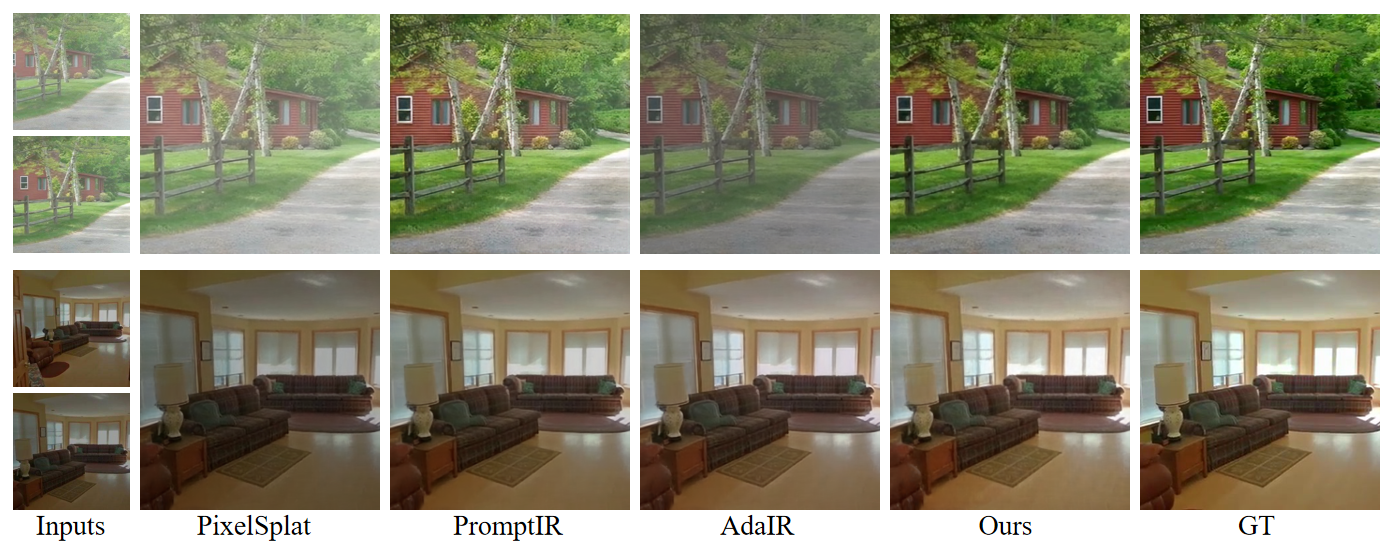
\includegraphics[width=1.0\textwidth]{fig_sup.png} % Reduce the figure size so that it is slightly narrower than the column. Don't use precise values for figure width.This setup will avoid overfull boxes.
\caption{Additional qualitative comparison. The visual quality of our method outperforms restore before reconstruct methods. Visual examples in the first and second rows correspond to foggy and dark degradation scenes, respectively.}
\label{fig:vis_rgb}
\end{figure*}

\section{Additional Ablation Study}
Due to space limitations in the main text, we provide additional ablation experiments to demonstrate the effectiveness and rationality of the proposed method. Below, we present detailed descriptions of additional ablation studies and implementation details.

\paragraph{Ablation Study on GenDeg.}
Existing methods such as DegAE adopt a degradation-aware encoder to extract degradation embeddings from input images for restoration purposes, but these approaches typically rely on reconstruction loss alone. In contrast, our proposed GenDeg introduces two additional objectives: a contrastive loss to encourage discrimination between different degradation types and a classification loss to further promote semantic alignment with known degradation categories. Table~\ref{table_deg} presents an ablation study on the loss functions used in GenDeg, demonstrating that our design contribute significantly to performance.

\begin{table}[th!]
\centering
\begin{tabular}{ccc|ll}
\toprule
$\mathcal{L}_{\mathrm{rec}}$ & $\mathcal{L}_{\mathrm{con}}$ & $\mathcal{L}_{\mathrm{cls}}$ & PSNR  & SSIM   \\ \midrule
\checkmark                   &                  &                     & 21.87 & 0.7751 \\
\checkmark                   & \checkmark                &                     & 22.09 & 0.7816 \\
\checkmark                   &                  & \checkmark                   & 21.95 & 0.7810  \\
\checkmark                   & \checkmark                & \checkmark                   & 22.32 & 0.7869
\\ \bottomrule
\end{tabular}
\caption{Ablation study on training loss of GenDeg.}
\label{table_deg}
\end{table}


\paragraph{Ablation Study on MV-SSEM.}
In the MV-SSEM, we use a semantic prompt pool of size $K$ to cluster tokens based on semantic similarity. We conduct an ablation study by varying the number of semantic prompts ($K=32, 64, 128$), as shown in Table~\ref{tab:prompt_k}. The results indicate that $K=64$ yields the best performance. A smaller $K$ leads to overly coarse semantic grouping, while a larger $K$ causes excessive fragmentation, making cross-view aggregation unstable. These experientments validate our design choice for prompt pool size.

We also conduct an ablation study to evaluate the impact of the internal dimensionality of each semantic prompt, denoted as $d_{\text{inner}}$, on the final performance. As shown in Table~\ref{tab:prompt_dim}, increasing the dimensionality from 32 to 128 leads to consistent improvements. However, further increasing beyond 128 brings no significant gain. Therefore, we choose $d_{\text{inner}} = 128$ in our implementation to balance representation capacity and computational cost.

\begin{table}[ht]
\centering
\begin{tabular}{c|ccc}
\toprule
Prompt Number ($K$) & PSNR & SSIM  & LPIPS \\
\midrule
32  & 21.93 & 0.7804 & 0.2513 \\
128 & 21.75 & 0.7717 & 0.2488 \\
64  & \textbf{22.32} & \textbf{0.7869} & \textbf{0.2443} \\
\bottomrule
\end{tabular}
\caption{Ablation study on $K$. }
\label{tab:prompt_k}
\end{table}

\begin{table}[ht]
\centering
\begin{tabular}{c|ccc}
\toprule
Prompt Dim ($d_{\text{inner}}$) & PSNR & SSIM  & LPIPS \\
\midrule
32   & 21.95 & 0.7798 & 0.2564 \\
64   & 22.24 & 0.7847 & 0.2471 \\
128  & \textbf{22.32} & \textbf{0.7869} & \textbf{0.2443} \\
\bottomrule
\end{tabular}
\caption{Ablation on $d_{\text{inner}}$.}
\label{tab:prompt_dim}
\end{table}


% \bibliography{aaai2026}

% \end{document}

\end{document}
